\documentclass[11pt]{article}

\usepackage[margin=1in, letterpaper]{geometry}
\usepackage{parskip}

\usepackage{amsthm, amsmath, amssymb}
\usepackage[pdftex]{graphicx}
\usepackage{hyperref}

\usepackage{enumerate} % For use of (a), (b), et cetera
\usepackage{booktabs}
\usepackage[margin=10pt, labelfont=bf, labelsep=period,
justification=justified]{caption}


% The following metadata will show up in the PDF properties
\hypersetup{
	colorlinks = true,
	urlcolor = black,
	pdfauthor = {Aaron Tran},
	pdfkeywords = {berkeley},
	pdftitle = {Astro 121, UG Radio Lab, Lab 2 - \today},
%	pdfsubject = {},
	pdfpagemode = UseNone
}

% Don't indent paragraphs
\setlength\parindent{0em}

% ===============
% Useful commands
% ===============
\newcommand {\mt}{\mathrm}
\newcommand {\unit}[1]{\; \mt{#1}}
\newcommand {\ints}{\mathbb{Z}}
\DeclareMathOperator{\sinc}{sinc}
% http://vemod.net/typesetting-units-in-latex

% ==========================
% Document specific commands
% ==========================

\begin{document}

% =======
% Titling
% =======
\begin{center}
\Large{Signal processing techniques for digital down conversion}

\large
Aaron Tran \\
\today \\
Partners: David Galbraith, Vikram Iyer \\
Prof. Aaron Parsons, GSI Karto Keating, UGSI Baylee Bordwell
\end{center}

% ========
% Abstract
% ========
\section*{Abstract}

We review Nyquist aliasing, analog and digital heterodyning, and finite impulse
response (FIR) filter design for use in an FPGA-based digital down converter.

Blah blah.

% ============
% Introduction
% ============
\section{Introduction}

Motivation blah.

Roadmap for the paper.
We demonstrate the Nyquist criterion, among other salient considerations
(spectral leakage, spectral resolution, aliasing). 

% ==================
% Aliasing and stuff
% ==================
\section{Background material}

\subsection{Aliasing and spectral leakage}

Digitizing of analog signals requires discretization with (1) finite sampling
rate and (2) finite sampling time.  These effects give rise to aliasing and
spectral leakage respectively; in the limit of infinitely fast sampling and
infinite sampling time, we recover the continuous Fourier transform.

Qualitatively, aliasing occurs when we cannot sample rapidly enough to capture
the input frequency.  However, we still obtain information about this frequency
component -- it is aliased (or, mirrored, folded) to a lower frequency
determined by both the input and sampling frequencies.  Spectral leakage occurs
our input frequencies are not ``tuned'' to the finite sampling time, such that
a fractional number of cycles occur in the sampling time.  Then, adjacent
frequencies are necessary to represent this behavior.

Discrete sampling at time intervals $T$ is equivalent to multiplying the input
signal with a ``train'' of Dirac delta impulses with spacing $T$:
\[
    g(t) = \sum_{n = -\infty}^\infty \delta (t - n T)
\]
This corresponds to convolving the frequency domain input signal with another
impulse train of spacing $f_{\mt{samp}} = 1/T$ (proof omitted).  The input
signal's frequency spectrum is then ``cloned'' in frequency space with a
periodicity $1/T$.  If the input signal's frequency spectrum falls within the
bandwidth $-f_{\mt{samp}} / 2, +f_{\mt{samp}} / 2$, the cloned frequency
spectra will be independent; each spectrum fits neatly into a bandwidth smaller
than $1/T$. The frequency $f_{\mt{samp}} / 2$ is known as the Nyquist
frequency, which I denote by $f_N$.  If the input signal has frequency
components above $f_N$, the cloned spectra begin to overlap.  Higher frequency
components appear in the bandwidth $[0, +f_{\mt{samp}} / 2]$ at frequencies
$n f_{\mt{samp}} - f$ ($f$ is the original signal frequency, and $n \in \ints$
such that $(n f_{\mt{samp}} - f) \in [-f_N, f_N]$.  Note that we may also
consider negative frequencies ($f < 0$) in this formulation.

Sampling for a finite time $\tau$ is equivalent to multiplying our input signal
by a rectangular function:
\[
    g(t) =
    \begin{cases}
        1 &\text{if } x \in [-\tau/2, \tau/2] \\
        0 &\mt{if } |x| > \tau/2
    \end{cases}
\]
This corresponds to convolving the frequency domain input signal with a sinc
function, where we define $\sinc(x) = \sin(\pi x)/(\pi x)$:
\[
    G(f) = \tau \,\frac{\sin (\pi f \tau)}{\pi f \tau}
         = \tau \,\sinc (f \tau)
\]
Consequently, input at a single frequency (e.g. a sinusoid) is smeared out in
frequency space (e.g., Figure 1a).  A longer sampling window will reduce the
smearing, causing the side frequencies to drop off more rapidly (corresponding
to a sharper sinc function).  For certain frequencies, spectral leakage is
sharply reduced or non-existent when the zero crossings of the convolving sinc
correspond to the frequency bins of the applied discrete Fourier transform.

I will avoid explicitly pointing out the presence of spectral
leakage for the rest of this report (excepting Figure 1), as nearly all
frequency/power spectra plotted exhibit spectral leakage.

% =====================
% Aliasing measurements
% =====================
\subsection{Aliasing measurements}

We illustrate these phenomena (aliasing in particular) by sampling an analog
signal of varying frequency ($f_{\mt{sig}}$) at fixed sampling frequency
$f_{\mt{samp}} = 10 \unit{MHz}$.
We collect 1024 samples and plot the corresponding waveforms and power spectra
in Figure 1; power spectra are calculated using the usual discrete Fourier
transform.
Here I omit the power spectra for negative frequencies ($-5$ to $0
\unit{MHz}$), which simply mirrors the spectra for positive frequencies as our
signal is real-valued.

% This is super hacky.  Ugh.
\newpage
\begin{figure}[!ht]
    \centering
    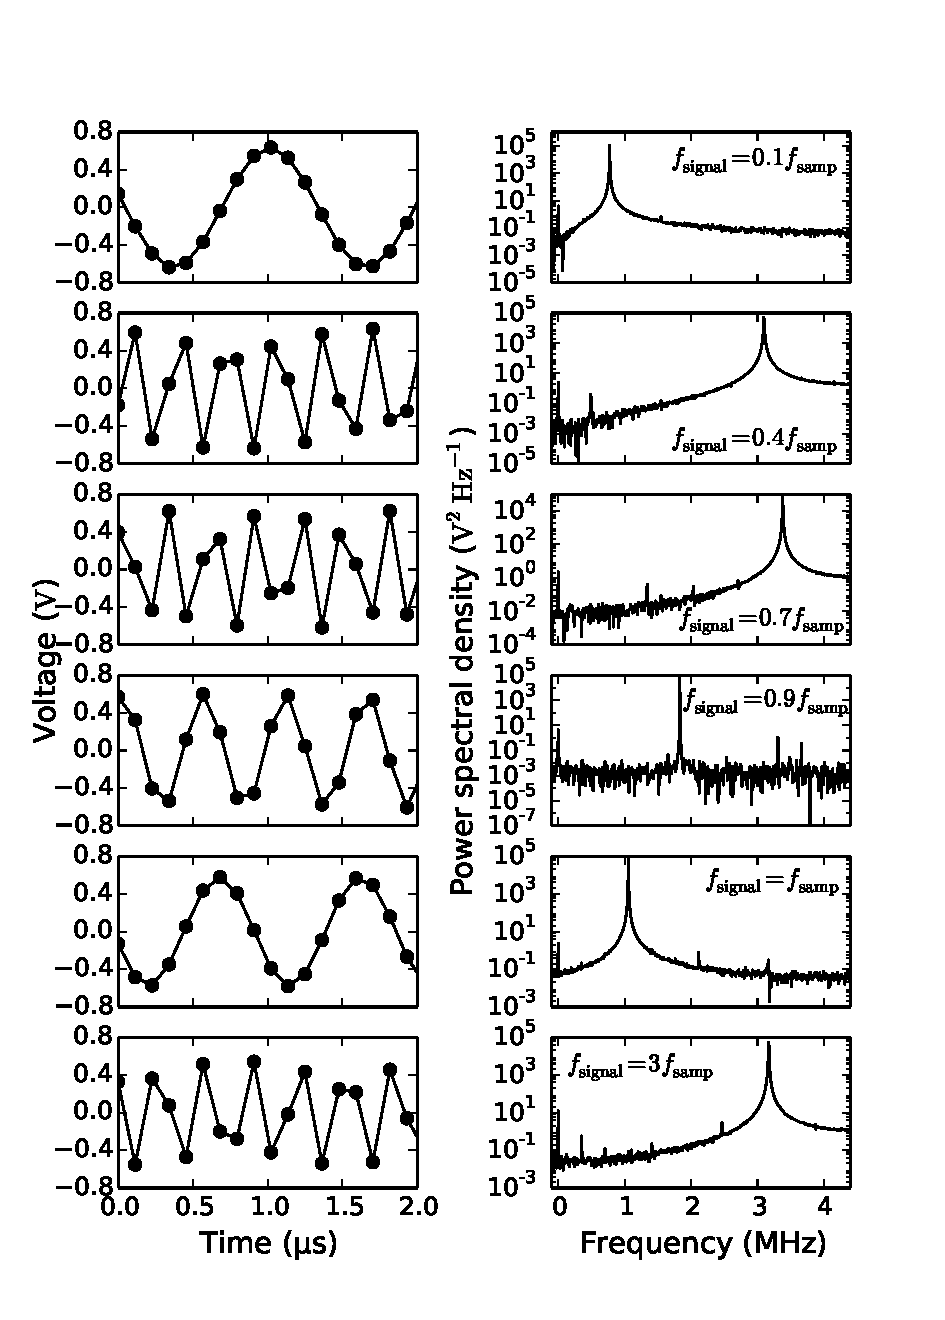
\includegraphics[scale=0.95]{scripts/nyquist_plots.pdf} \\
    \caption{Sampled waveforms (left) and power spectra (right). The
    Nyquist frequency is 5 MHz; I omit the power spectra for negative
    frequencies $-5$ to $0 \unit{MHz}$.
    The input signal frequencies are (a) 0.88 MHz, (b) 3.52 MHz, (c) 6.16 MHz,
    (d) 7.92 MHz, (e) 8.8 MHz, (f) 26.4 MHz;
    the sampled signals have spectra peaks at (a) 0.87 MHz,
    (b) 3.52 MHz, (c) 3.83 MHz, (d) 2.09 MHz, (e) 1.21 MHz, (f) 3.61 MHz.
    Plots (c)--(e) display aliasing.}
\end{figure}
\newpage

Spectral leakage is visible throughout Figures 1a--f; aliasing is present in
Figures 1c--f.  The spectrum in Figure 1d has relatively small
spectral leakage; this appears to have occured by chance, as the uncertainties
in our input/sampling frequencies are comparable to or larger than the
frequency resolution ($f_{\mt{samp}} / 1024 \approx 10 \unit{kHz}$) of our
discrete Fourier transform.

As our input frequencies are known \emph{a priori}, we may predict where
aliased frequencies should appear in our calculated power spectra.
For example, Figure 1c has $f_{\mt{sig}} = 6.16 \unit{MHz}$; we expect the
aliased signal to appear at $f_{\mt{samp}} - f_{\mt{sig}} = 3.84 \unit{MHz}$.
Table 1 gives the predicted and measured frequencies for Figure 1, which agree
within uncertainty.

\begin{table}[t]
\centering
\caption{Comparison of predicted and observed frequency aliasing.
Predicted uncertainties are estimated from maximum observed fluctuation in
oscilloscope measurements of signal period; we are unable to estimate and
include error in sampling frequency.
Observed uncertainty is set to frequency resolution $\sim 10 \unit{kHZ}$, set
by discrete Fourier transform (number of samples and sample rate).}
\begin{tabular}{@{}rrr@{}}
    \toprule
    & \multicolumn{2}{c}{$f_{\mt{aliased}} \unit{(MHz)}$} \\
    \cmidrule(l){2-3}
    $f_{\mt{sig}} \unit{(MHz)}$ & predicted & observed \\
    \midrule
    0.88 & $0.88 \pm 0.003$ & $0.87 \pm 0.01$ \\
    3.52 & $3.52 \pm 0.02$ & $3.52 \pm 0.01$ \\
    6.16 & $3.84 \pm 0.08$ & $3.83 \pm 0.01$ \\
    7.92 & $2.08 \pm 0.04$ & $2.09 \pm 0.01$ \\
    8.80 & $1.20 \pm 0.03$ & $1.21 \pm 0.01$ \\
    26.4 & $3.60 \pm 0.3$ & $3.61 \pm 0.01$ \\
    \bottomrule
\end{tabular}
\end{table}

For the remainder of this study, we mix and sample signals with information
carried below the Nyquist frequency.

% =======================
% Heterodyning background
% =======================
\subsection{Signal heterodyning}

We now consider heterodyning: the process of mixing (multiplying) two signals
to obtain a frequency-shifted output signal.  Heterodyning is commonly used to
downconvert a high frequency radio signal to one of lower frequency with the
same information content; at a lower frequency, the signal is easier to sample,
filter, or otherwise manipulate.  We mix a real-valued input signal of
frequency $f_{\mt{sig}}$ with a local oscillator signal of frequency
$f_{\mt{LO}}$.  The mixer outputs a signal with frequencies $f_{\mt{LO}} \pm
f_{\mt{sig}}$.
 
Single/double sidebands are most relevant to AM signal processing with 
$f_{\mt{sig}} \ll f_{\mt{LO}}$, which produces two bands to the left and
right of $f_{\mt{LO}}$.  This assumes a single mixing frequency $f_{\mt{LO}}$.
Here we consider a slightly different situation.  Typically we choose
$f_{\mt{LO}}$ to be close to $f_{\mt{sig}}$, so that the difference
$f_{\mt{LO}} - f_{\mt{sig}}$ is significantly smaller than either
$f_{\mt{sig}}$ or $f_{\mt{LO}}$ (say, by an order of magnitude, and the sum
product $f_{\mt{LO}} + f_{\mt{sig}}$ is then about twice the size of each input
frequency.

We define double sideband (DSB) mixing as heterodyning with local oscillator
frequencies $\pm f_{\mt{LO}}$, which outputs frequencies $\pm f_{\mt{LO}} \pm
f_{\mt{sig}}$ (four tones in total).  Mixing with two frequencies (e.g. by
using a real-valued signal) creates redundant information, manifest in the
reflection symmetry of the output signal's frequency spectrum about $f = 0$.
We then define single sideband (SSB) mixing as heterodyning with a single local
oscillator frequency $f_{\mt{LO}}$, as given above.  Importantly, this still
gives rise to both sum and difference frequencies -- we have only removed
redundant information.

We then define upper and lower sidebands as the output frequencies
associated with $+f_{\mt{LO}}$ and $-f_{\mt{LO}}$ respectively.  If
$f_{\mt{sig}} < f_{\mt{LO}}$, these sidebands are associated with positive and
negative frequency components only.  Filtering will be necessary to obtain,
e.g. only difference or sum frequencies for further manipulation.

% ==============
% Mixing methods
% ==============
\section{Methods and materials}

Here we consider analog double sideband mixing and digital single/double
sideband mixing.  We generate analog signals using a Stanford Research Systems
DS345 function generator and perform analog mixing with a Mini-Circuits ZAD-1
mixer.  We perform digital mixing using a ROACH processing board, produced by 
the radio instrumentation collaboration CASPER.  The ROACH implements single
and double sideband mixing through an analog-digital converter (ADC) connected
to a field-programmable gate array (FPGA).  Input signals to the ROACH ADC are
sampled at $200 \unit{MHz}$, then mixed with a digital local oscillator and
output on the FPGA.  The FPGA hardware design is pre-compiled using the
Berkeley Operating system for Re-Programmable Hardware (BORPH).

To assess the effects of mixing, we discretely sample both analog and digital
mixing outputs.  We record 1024 samples of analog mixer output at $10
\unit{MHz}$ using a PC-based ADC; we take 2048 samples of digital mixer output
at $200 \unit{MHz}$ from the ROACH FPGA's block memory.

We additionally characterize a digital down converter implemented on the ROACH
board's FPGA, composed of a SSB mixer and an 8-tap finite impulse
response (FIR) filter.  We verify correct SSB mixer and filter operation by
varying local oscillator (SSB mixer) frequency for fixed input frequency.

\subsection{FIR filter implementation}

We attempt to implement a 5/8 FIR filter but ultimately use a 1.6/8 filter.
We first compute the continuous Fourier transform of our frequency-domain
filter function, then compute filter coefficients at discrete times.  In
frequency space, our desired filter function $G(f)$ is:
\[
    G(f) =
    \begin{cases}
    1   &   \mt{if } |f| < 62.5 \unit{MHz} \\
    0   &   \mt{if } |f| \geq 62.5 \unit{MHz}
    \end{cases}
\]
Apply an inverse Fourier transform (neglecting normalization).
Here $\omega_N = 2\pi (100 \unit{MHz})$ denotes the Nyquist frequency.
\begin{align*}
    g(t) &= \mathcal{F}^{-1}\left( G(f) \right) \\
         &= \int_{-5/8 \omega_N}^{5/8 \omega_N} e^{i\omega t} d\omega \\
         &= \cdots \\
         &\propto \frac{\sin \left( \frac{5}{8} \omega_N t \right)}
            {\frac{5}{8} \omega_N t}
\end{align*}
Now we may discretize $t = n / f_{\mt{samp}} = n \pi / \omega_N$, where
$n\in\ints$ counts each sample time.  As before, we define $\sinc(x) =
\sin(\pi x) / (\pi x)$.  Then we obtain an expression for the discretized,
time-domain filter function:
\[
    g(n) = \sinc \left( \frac{5}{8} n \right)
         = \frac{\sin \left( \frac{5}{8} \pi n \right)}
         {\frac{5}{8} \pi n}
\]
Our 8 tap filter coefficients are $g(n)$ for $n=-4, -3, \cdots 3$; the values
are tabulated in Table 2.

Regrettably, we miscalculated our coefficients by using $\sinc(x) = \sin (x)/x$
on Wolfram\textbar Alpha.  This corresponds to changing our filter cut-off from
$5/8$ to $5/(8\pi) \approx 1.6/8 \approx 0.2$.  We performed our FIR filter
analysis using these altered coefficients, also given in Table 2.

\begin{table}[t]
\centering
\caption{FIR filter coefficients for desired 5/8 filter and implemented 1.6/8
filter}
\begin{tabular}{@{}rrr@{}}
    \toprule
    FIR coeff. & 5/8 filter & 1.6/8 filter \\
    \midrule
    $c_0$ &  $0.12732$ & $0.23939$ \\
    $c_1$ & $-0.06496$ & $0.50885$ \\
    $c_2$ & $-0.18006$ & $0.75919$ \\
    $c_3$ &  $0.47053$ & $0.93616$ \\
    $c_4$ &  $0.99999$ & $0.99999$ \\
    $c_5$ &  $0.47053$ & $0.93616$ \\
    $c_6$ & $-0.18006$ & $0.75919$ \\
    $c_7$ & $-0.06496$ & $0.50855$ \\
    \bottomrule
\end{tabular}
\end{table}

As a final exercise, we translate our FIR coefficients back into the frequency
domain to check the expected frequency response (Figure 2).  In Figure 2b, we
compute the 64 point filter response by padding FIR coefficients with zeros.

\begin{figure}[!htb]
    \centering
    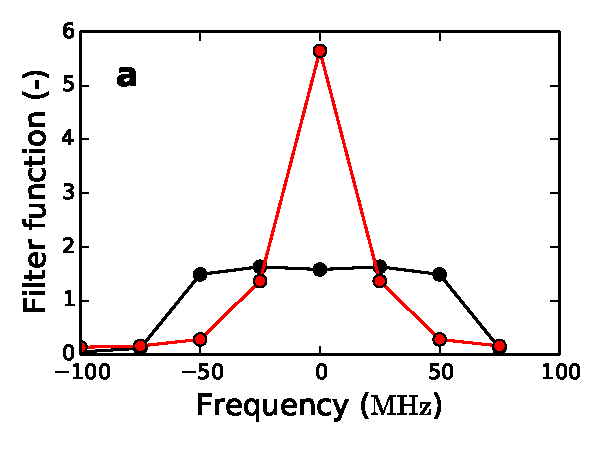
\includegraphics[scale=0.8]{scripts/FIR_filter_responses.pdf}
    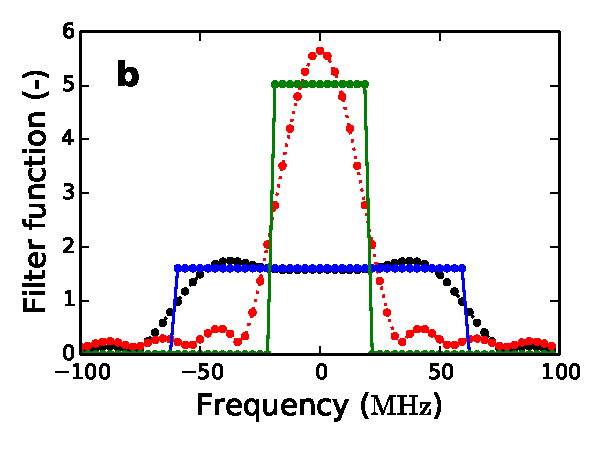
\includegraphics[scale=0.8]{scripts/FIR_filter_responses_fine.pdf}
    \caption{Predicted 8-tap FIR filter frequency responses.
    (a) Filter responses at 8 points, 1.6/8 filter in red, 5/8 filter in black
    (b) filter response at 64 points. Predicted responses for 1.6/8 and 5/8
    filters red, black as in (a); desired/ideal responses for 1.6/8 and 5/8
    filters in green, blue.  I apologize for the colorblind unfriendly color
    choices.}
\end{figure}

% =======
% Results
% =======
\begin{figure}[!ht]
    \centering
    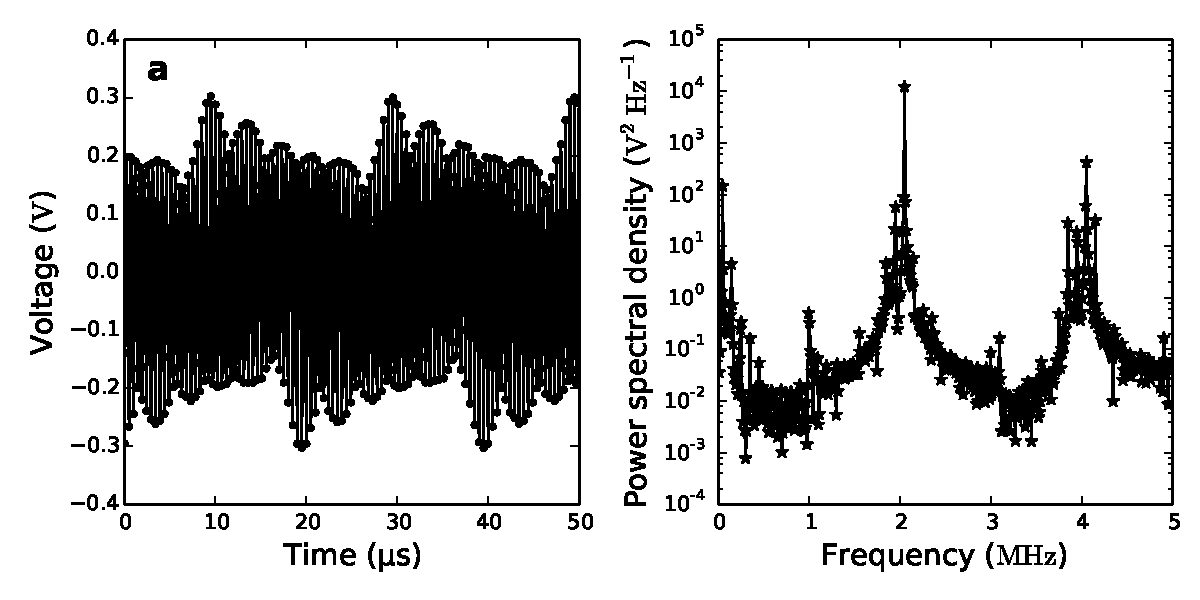
\includegraphics[scale=0.44]{scripts/analog_mixing_DSB_0.pdf} \\
    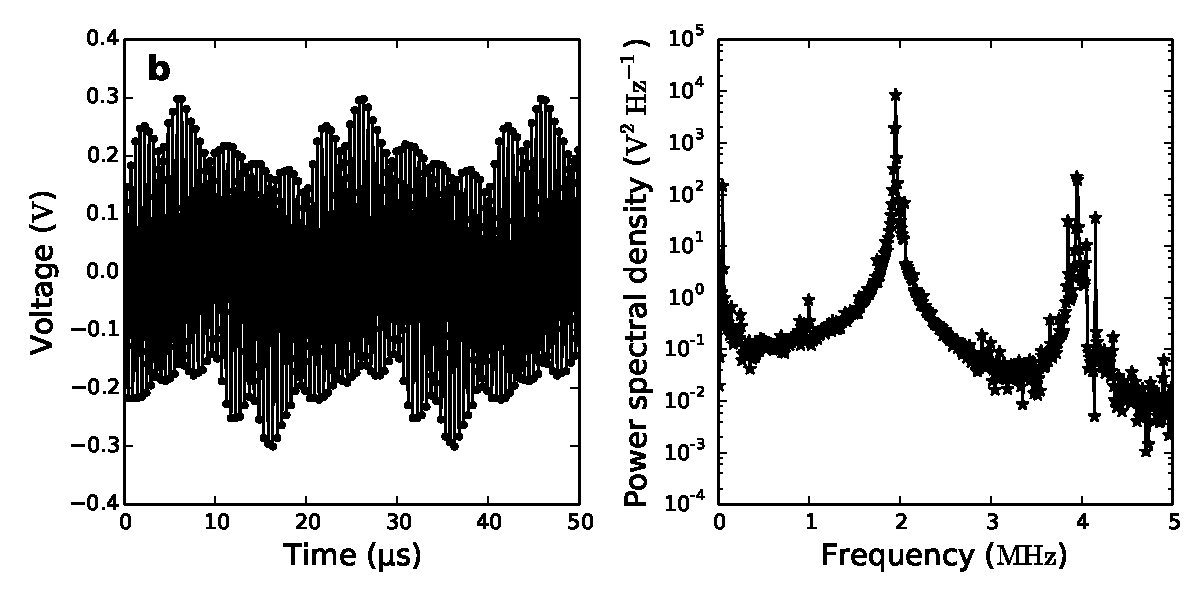
\includegraphics[scale=0.44]{scripts/analog_mixing_DSB_1.pdf} \\
    \caption{Analog mixing of two sinusoids with frequencies (a) $1, 1.05
    \unit{MHz}$; (b) $1, 0.95 \unit{MHz}$; time-domain signals plotted on left
    with corresponding power spectra on right.  Power spectra show peaks at
    $0.05 \unit{MHz}$, $2.05 \unit{MHz}$ (a), and $1.95 \unit{MHz}$ (b) as
    expected.  We are unable to explain peaks at $4.05 \unit{MHz}$ (a) and
    $3.95 \unit{MHz}$ (b).}
    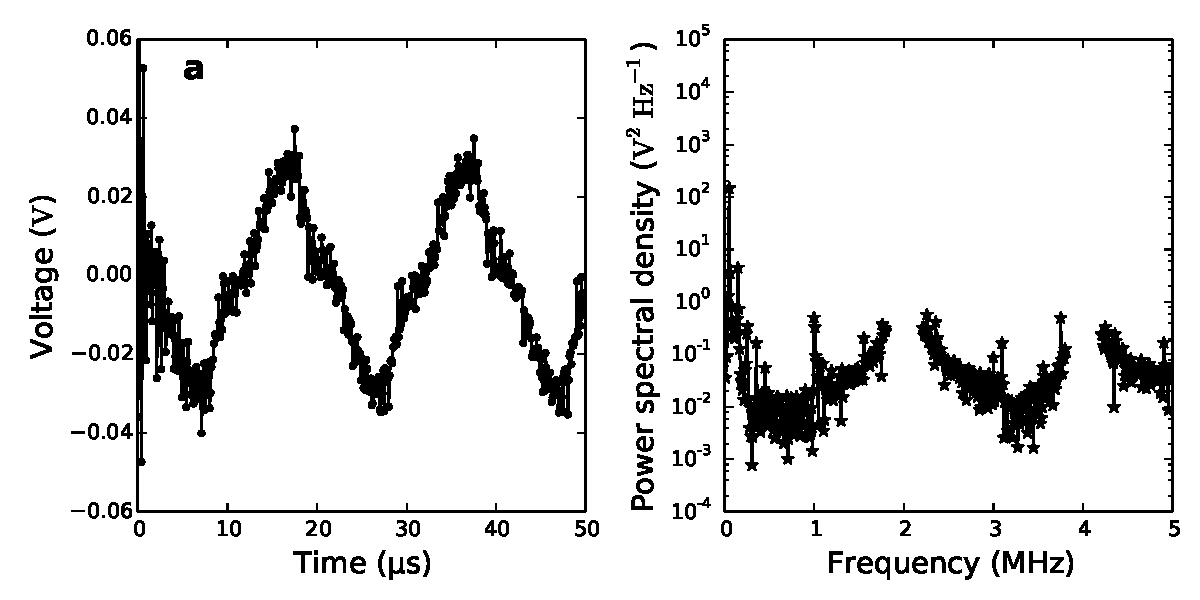
\includegraphics[scale=0.44]{scripts/analog_mixing_DSB_filtered_0.pdf} \\
    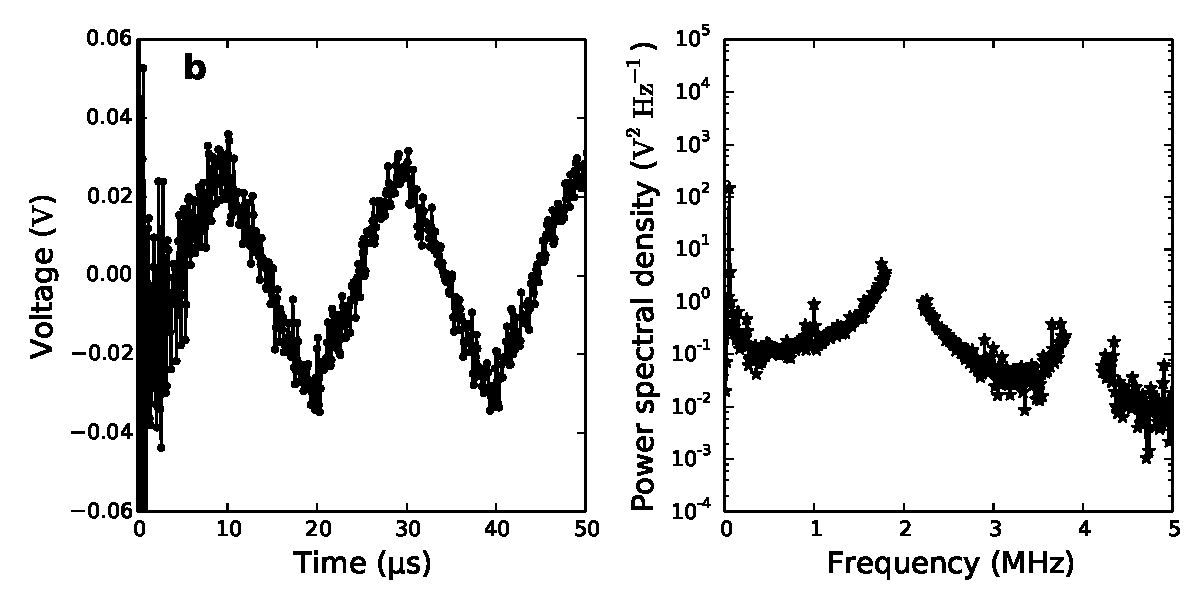
\includegraphics[scale=0.44]{scripts/analog_mixing_DSB_filtered_1.pdf} \\
    \caption{Fourier filtering of signals in Figure 3 allows recovery of $0.05
    \unit{MHz}$ frequency component.  Subfigures (a), (b) as in Figure 3.
    We zero all frequency components in $(1.8, 2.2) \unit{MHz}$ and
    $(3.8, 4.2) \unit{MHz}$ to leave only the $0.05 \unit{MHz}$ signal.}
\end{figure}

\section{Results}

\subsection{Double sideband mixing}

\subsubsection{Analog DSB}

We mix two real-valued sinusoids at $f_{\mt{LO}} = 1 \unit{MHz}$ and
$f_{\mt{sig}} = (1 \pm 0.05) \unit{MHz}$ using our Mini-Circuits analog mixer
and plot the time-domain and frequency-domain signals in Figure 3.  I omit the
power spectra for negative frequencies, which are mirror images of the spectra
for positive frequencies.  As expected, we observe signals at the sum and
difference frequencies $\pm f_{\mt{LO}} \pm f_{\mt{sig}}$; our input signal has
been cloned to two frequencies nearly two orders of magnitude apart.

The concepts of upper and lower sidebands as defined above are not so helpful
here.  In Figure 3a, the upper sideband has frequencies $2.05 \unit{MHz}$,
$-0.05 \unit{MHz}$ (not shown); the lower sideband has frequencies $0.05
\unit{MHz}$ and $-2.05 \unit{MHz}$ (not shown).  In Figure 2b, both positive
frequencies are associated with our upper sideband.

The power spectra also display unexpected tones at approximately $1,4
\unit{MHz}$.  A tone at about $0.95, 1, 1.05 \unit{MHz}$ may be due to a
weak DC offset that replicates the input signal frequencies when mixed.
However, we are at a loss to explain very strong tones at $3.95, 4.05
\unit{MHz}$.  All mixing products were expected to have frequencies less than
the Nyquist frequency; any aliasing or mixing giving rise to these tones must
be driven by an additional signal source that we have neglected.

In Figure 4, we manually apply a Fourier filter to the power spectra of Figure
3 to remove the frequency components near $2, 4 \unit{MHz}$ (setting the
relevant components to 0).  The inverse Fourier transform of the filtered
frequency spectrum gives the time-domain signals of Figure 4.  As expected, we
recover a signal that resembles a sine wave; we anticipate that given an
arbitrary signal with various components $f_{\mt{sig}}$, we should be able to
recover the signal shape.  Our recovered signal appears slightly more
triangular than expected, however.

\subsubsection{Digital DSB}

\begin{figure}[!t]
    \centering
    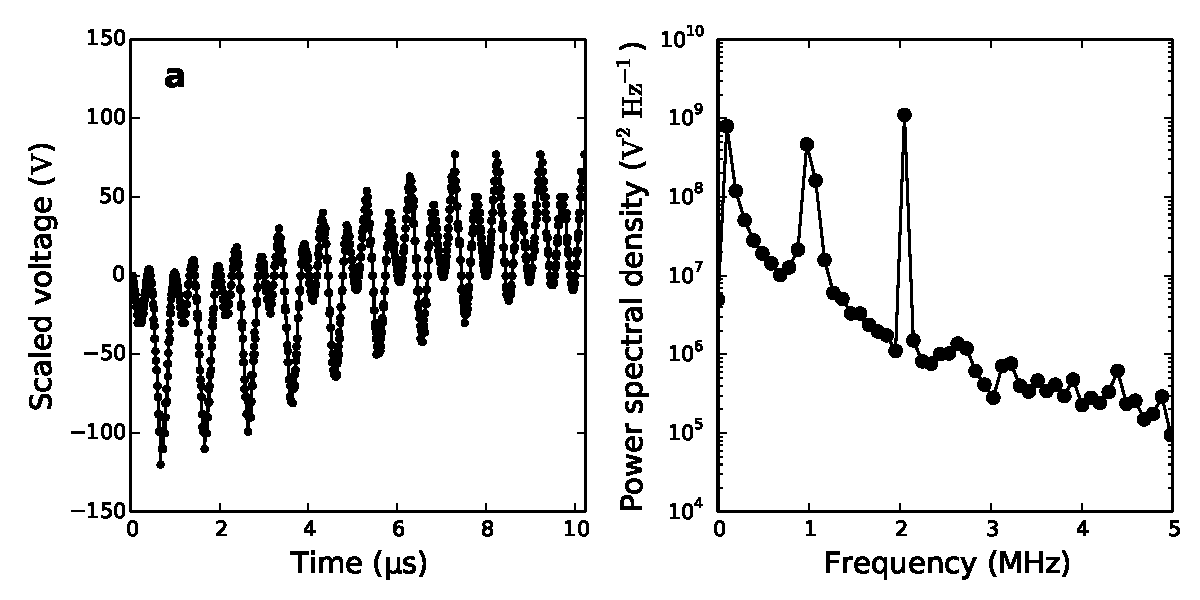
\includegraphics[scale=0.45]{scripts/digital_mixing_DSB_0.pdf} \\
    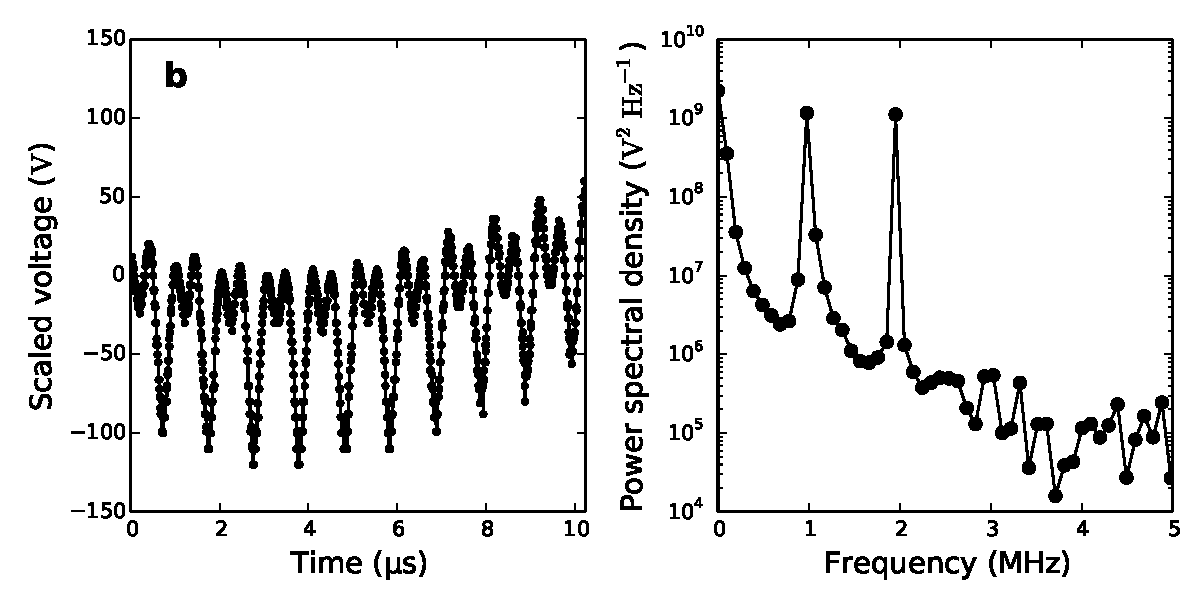
\includegraphics[scale=0.45]{scripts/digital_mixing_DSB_1.pdf} \\
    \caption{Digital DSB mixing of two sinusoids with frequencies (a) $1, 1.05
    \unit{MHz}$; (b) $1, 0.95 \unit{MHz}$ as in Figure 3 with corresponding
    power spectra on right.
    Power spectra show peaks at $0.05 \unit{MHz}$, $2.05 \unit{MHz}$ (a), and
    $1.95 \unit{MHz}$ (b) as expected.  Additional tones (unresolved and hence
    displayed as a single tone) at $1.0 \unit{MHz}$ are caused by introduction
    of DC offsets to analog signal inputs.}
\end{figure}

We repeated the analog DSB procedure for our FPGA-based digital DSB mixer and
plot the results in Figure 5; as before, we omit the redundant negative
frequency spectrum.  We observe mixing products at $0.05 \unit{MHz}$ and $1.95,
2.05 \unit{MHz}$ as before; however, decreased frequency resolution ($\sim 0.1
\unit{MHz}$) makes separating signals more difficult (e.g., the $0.05
\unit{MHz}$ signal in Figure 4b may be picked up in the $0 \unit{MHz}$ or $0.1
\unit{MHz}$ bin).

These signals, compared to those of Figures 3,4, do not carry frequency
components at $\sim 4 \unit{MHz}$.  We now observe very strong signals
at $\sim 1 \unit{MHz}$; these arise due to a DC offset introduced by the ROACH
ADC.  The DC offsets (frequency $0 \unit{MHz}$) in each signal are mixed with
the other signal's non-zero frequency components, cloning the input signals at
$0.95, 1, 1.05 \unit{MHz}$.

\subsection{Single sideband mixing}

We also use the ROACH to generate two local oscillator signals in quadrature
for single sideband mixing.  Given an input signal $f(t)$, the FPGA outputs
the signals $f(t) \cos (2\pi f_{\mt{LO}} t)$ and
$f(t) \sin (2\pi f_{\mt{LO}} t)$; we may multiply the $\sin$ signal by $+i$
and sum the outputs to obtain $f(t) \exp\left( 2\pi f_{\mt{LO}} t \right)$.
We demonstrate this with an input signal
$f_{\mt{sig}} = 10 \unit{MHz}$ mixed with signals at
$f_{\mt{LO}} = 6.25 \unit{MHz}$.  The expected mixing products are $\pm 10 +
6.25 \unit{MHz}$, or $-3.75, +16.25 \unit{MHz}$.  If the $\sin$ signal is
multiplied by $-i$, we will obtain $-16.25, +3.75 \unit{MHz}$ mixing products
instead, corresponding to our defined lower sideband.

\begin{figure}[!htb]
    \centering
    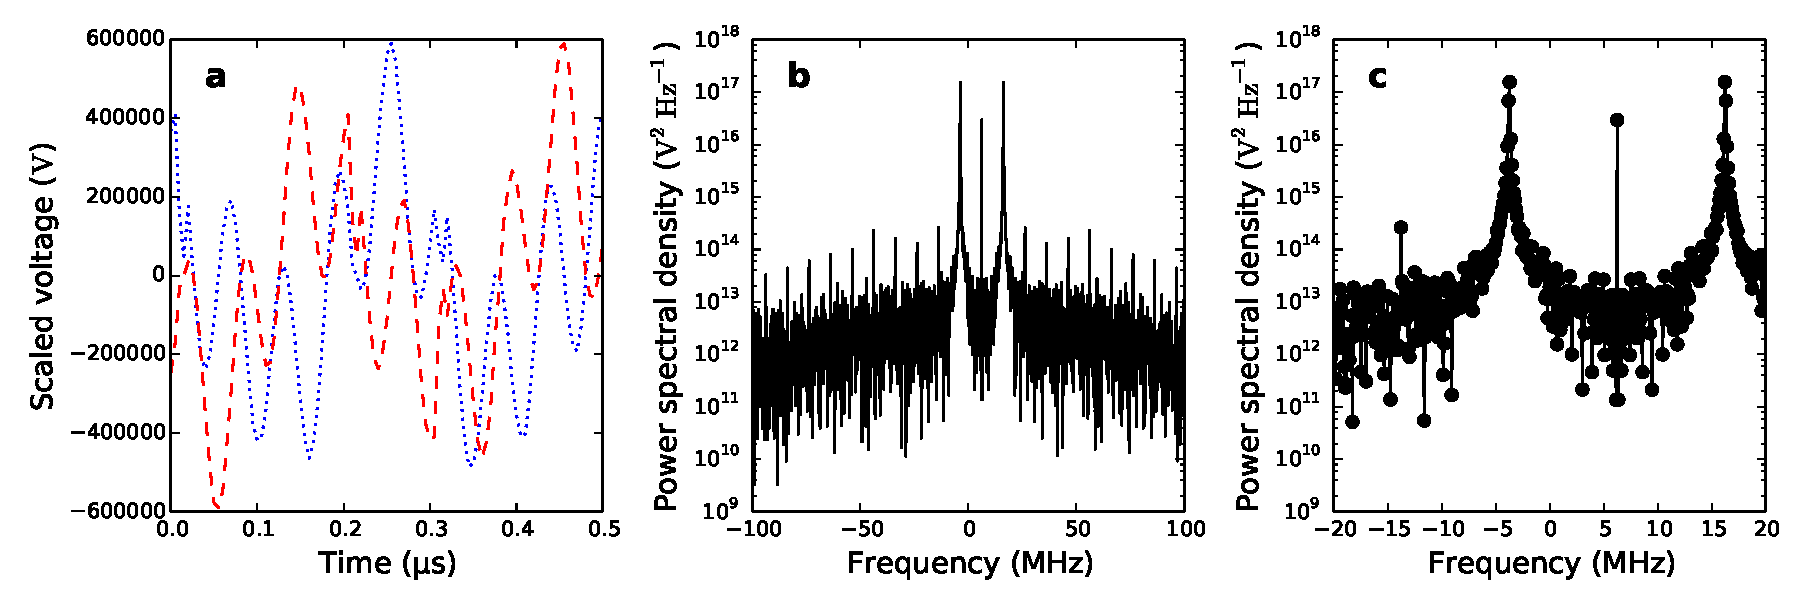
\includegraphics[width=\textwidth]{scripts/digital_mixing_SSB.pdf} \\
    \caption{Digital single sideband mixing with $f_{\mt{sig}} = 10\unit{MHz}$,
    $f_{\mt{LO}} = 6.25 \unit{MHz}$.  (a) Intermediate mixing products of input
    signal and $\cos(2\pi f_{\mt{LO}} t)$, $\sin(2\pi f_{\mt{LO}})$.  Cosine
    mixing product is dotted blue; sine mixing product is dashed red.
    (b) Power spectrum of fully mixed signal (see text).  Spectrum is not
    centered on $f=0$ (clearer in (c)).
    (c) Zoomed view of power spectrum in (b).  Only two mixing products are
    present as expected for SSB mixing.}
\end{figure}

As for the analog DSB signal, we attempt to Fourier filter out the higher sum
frequency in Figure 7.  The resultant real and complex time-domain signals are
plotted in Figure 7a.

If we had an ideal continuous Fourier transform, we might expect the
Fourier filtered time-domain signal to look like
$\exp\left[ 2\pi i \left( f_{\mt{LO}} - f_{\mt{sig}} \right) \right]$.
Our filtered signal appears to oscillate rapidly (every timestep), but the
overlying amplitude modulation appears to have frequency consistent our
measured difference frequency $-3.71 \unit{MHz}$ if two lobes are counted as a
single cycle.  The oscillation does not disappear even if we Fourier filter to
get only the peak at $-3.71 \unit{MHz}$.  We are unable to explain this
filtered behavior currently, and it does not seem obvious which signal leads
the other (to check that the waveforms carry a negative frequency).

\begin{figure}[!htb]
  \centering
  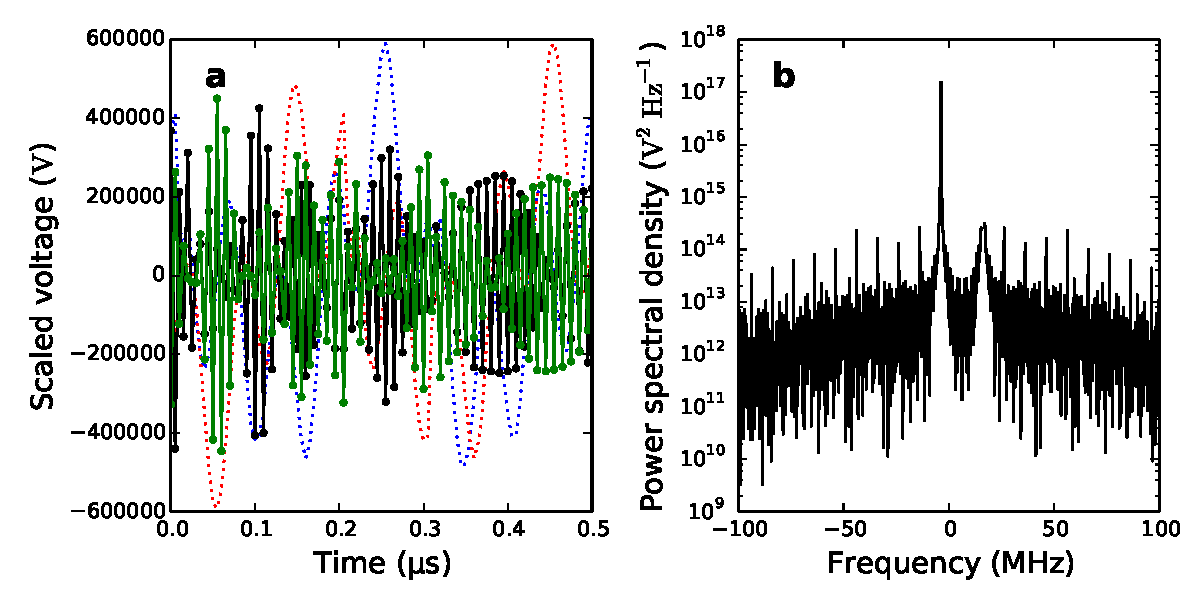
\includegraphics[scale=0.5]{scripts/digital_mixing_SSB_filtered.pdf}\\
  \caption{Fourier filtering of digital SSB mixer output. (a) Real (black),
  imaginary (green) components of filtered signal in time-domain; original
  cosine/sine mixing products plotted in blue, red dots in background.
  (b) Fourier filtered power spectra; frequency components in $(15.5, 17)
  \unit{MHz}$ are set to zero.}
\end{figure}

\subsection{Digital down converter}

We feed a $30 \unit{MHz}$ signal into our digital down converter (DDC) and
obtain the DDC's frequency response by varying the SSB mixer's local oscillator
frequency ($7.8$ to $46.9 \unit{MHz}$ in intervals of $\approx 7.8 \unit{MHz}$.

For lack of time, Figure 8 simply plots a melange of power spectra output from
our DDC.
Qualitatively, the noise and sum/difference frequencies appear to be attenuated
as expected, although we cannot confirm that signals fed into our FIR filter
have equal or comparable amplitudes.

\begin{figure}[!htb]
    \centering
    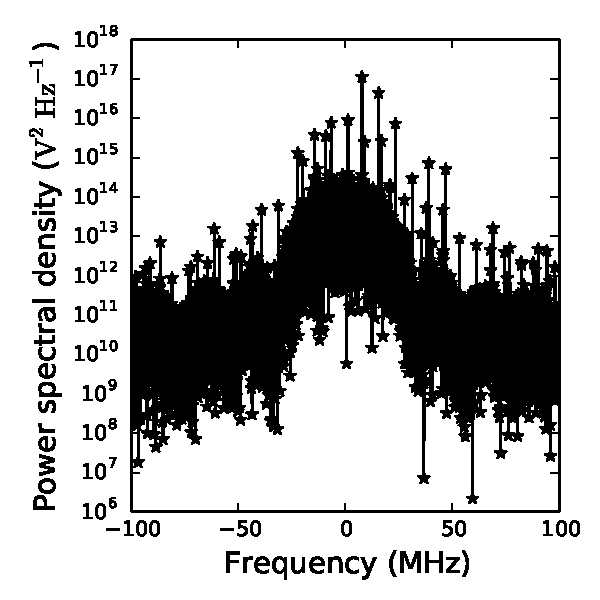
\includegraphics[scale=0.7]{scripts/DDC_response_log.pdf}
    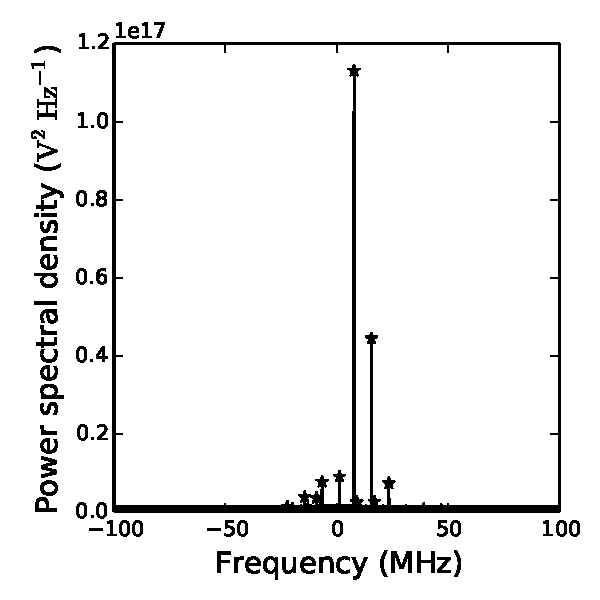
\includegraphics[scale=0.7]{scripts/DDC_response_lin.pdf}
    \caption{(a, left) Melange of DDC outputs; (b, right) same as (a) but
    plotted with logarithmic power spectral density.}
\end{figure}

\section{Discussion}

\subsection{Comparison of analog/digital SSB/DSB mixers}

Advantages and disadvantages of digital, analog SSB/DSB mixing.  Cost,
efficiency, discretization artifacts.  Neither analog nor digital processing
techniques are perfect, although digital is often very convenient.

Effective digital SSB mixing relies on the ability to generate two local
oscillator components with an accurate $\pi/2$ phase offset.  Figure 9
demonstrates how a small deviation from the $\pi/2$ offset (here, $\pi/2 + 0.2$
radians) re-introduces the complementary sideband's signals and reduces the
utility of the SSB mixer.

\begin{figure}[!htb]
    \centering
    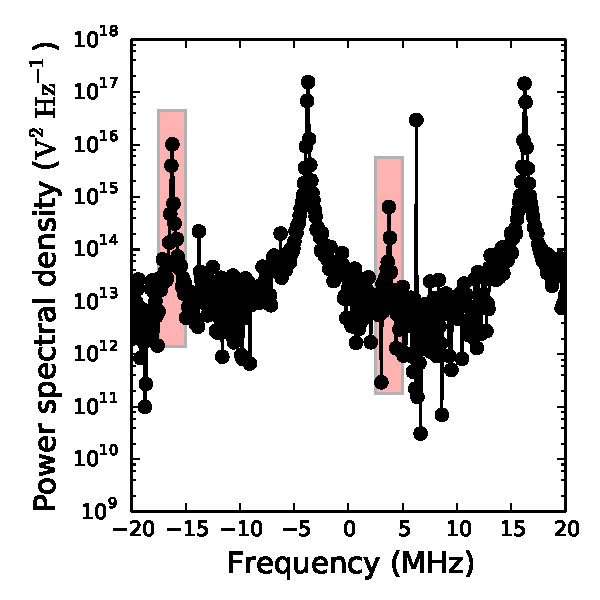
\includegraphics[scale=0.7]{scripts/digital_mixing_SSB_offset.pdf} \\
    \caption{Digital mixing of two local oscillator signals, slightly offset
    from $\pi/2$ phase shift, fails to achieve complete SSB mixing.  Two tones
    associated with DSB mixing reappear (red boxes).}
\end{figure}

\subsection{FIR filter design}

In essence, we must trade longer integration time (more taps) for sharper
filter responses.  We may choose different windows (e.g., triangular, Hamming,
et cetera) to obtain different frequency responses, depending on whether we
seek to obtain a flatter passband or sharper roll-off.  The considerations are,
of course, analogous to those in analog filter design.

\section{Conclusion}

Yay digital signals.

\section{Acknowledgments}

I thank Vikram for kindly elucidating various aspects of digital signal
processing.  Baylee, Karto, and Aaron answered and explained myriad questions.

\section{Electronic supplement}

All data and data analysis scripts (iPython notebooks) are stored on the
repository:\\
\href{https://github.com/aarontran/ay121}
{https://github.com/aarontran/ay121/lab2/}.

\end{document}
